\documentclass[preprint]{elsarticle}

%%%%%%%%%%%%%%%%%%%%%%%%%%%%%%%%%%%%%%%%%%%%%%%%%%%%%%%%%%%%%%%%%%%%%%
% Maths

\usepackage{amsmath}
\usepackage{wasysym}

% not perfect but works...
\newcommand{\mathup}{\mathrm}

\usepackage{siunitx}
\sisetup{detect-all=true,number-mode=math,list-units=single}
\DeclareSIUnit{\rpm}{rpm}

% Macros
\newcommand{\TR}{\mathup{T}}

\newcommand*{\diffdchar}{\mathrm{d}}
\newcommand*{\dd}{\mathop{\diffdchar\!}}

%%%%%%%%%%%%%%%%%%%%%%%%%%%%%%%%%%%%%%%%%%%%%%%%%%%%%%%%%%%%%%%%%%%%%%
% Figures & graphics
\usepackage{graphicx}

% \usepackage[colorlinks,citecolor=black,filecolor=black,linkcolor=black,urlcolor=black]{hyperref}
% \usepackage[left=3cm, right=3cm, top=2.5cm, bottom=3.5cm]{geometry}

\usepackage{calc}
\usepackage{booktabs}
\usepackage{enumitem}

\usepackage[displaymath]{lineno}
\linenumbers

\usepackage{array}
\newcolumntype{L}[1]{>{\raggedright\let\newline\\\arraybackslash\hspace{0pt}}p{#1}}

\bibliographystyle{elsarticle-num-names}

%%%%%%%%%%%%%%%%%%%%%%%%%%%%%%%%%%%%%%%%%%%%%%%%%%%%%%%%%%%%%%%%%%%%%%

\begin{document}

\begin{frontmatter}
  \title{Improved linearised models of wind turbine aerodynamics and control
    system dynamics using harmonic linearisation}

  \author[cued]{Richard C Lupton\corref{cor1}} \ead{rcl33@cam.ac.uk}

  \author[cued]{Robin S Langley} \ead{rsl21@cam.ac.uk}

  \cortext[cor1]{Corresponding author}

  \address[cued]{Department of Engineering, University of Cambridge, Trumpington
    St, Cambridge, CB2 1PZ, UK}

  \begin{abstract}
    Where non-linearities are not too strong, linearised frequency-domain
    approaches offer fast calculations, which can be valuable for preliminary
    design of wind turbine blades, foundations and floating platforms. But the
    aerodynamic and control system behaviour of a wind turbine is noticeably
    non-linear. Here we show for the first time that the technique of harmonic
    linearisation can reduce error in the approximation of aerodynamic and
    control system non-linearities, compared to the more common tangent
    linearisation. After deriving the linearised models, comparing linearised
    results to non-linear simulations for the NREL 5MW turbine shows that: (1)
    harmonic linearisation captures aero-elastic effects and non-linearity in
    aerodynamic forces, giving a 2--4x reduction in error compared to the
    tangent linearisation; (2) harmonic linearisation can capture non-linear
    wake dynamics; and (3) the torque and pitch controller behaviour can be
    approximated with good results away from the rated wind speed but with some
    challenges when the two controllers interact. Further improvements in the
    linearised model of the control system have been identified. By improving
    the accuracy of linearised models, harmonic linearisation is a promising
    means to extend the applicability of frequency-domain approaches for initial
    design and optimisation of wind turbines.
  \end{abstract}

\begin{keyword}
  wind energy \sep
  aerodynamic loads \sep
  frequency-domain modelling \sep
  harmonic linearisation \sep
  equivalent linearisation \sep
  non-linearity
\end{keyword}
\end{frontmatter}

\linenumbers

\section{Introduction}
\label{sec:introduction}

\begin{figure}
  \centering
  \includegraphics{figures/thrust_lin_example.pdf}
  \caption{Non-linearity is significant in the aerodynamic loading on a wind
    turbine. This example shows the thrust on one rotor annulus, calculated from
    a Blade Element Momentum (BEM) model. The tangent and harmonic
    linearisations of the thrust are shown, with all inputs held constant apart
    from a sinusoidal variation in wind speed. Left: as a function of wind
    speed. Right: as a function of time.}
  \label{fig:thrust}
\end{figure}

\begin{figure}
  \centering
  \includegraphics{figures/torque_nonlinearity}
  \caption{Examples of the response of the torque controller to harmonic
    variations in generator speed. The example at the left is mildly non-linear
    at the corners of the torque curve. For the example in the middle the
    underlying behaviour is quadratic, but over the range shown it is well
    approximated by the linear solution. The example at the right is highly
    non-linear.}
\label{fig:torque-nonlinearity}
\end{figure}

There are many sources of non-linearity in wind turbines. Some non-linearities
can reasonably be neglected for some purposes, such as structural non-linearity
\citep{lupton_complex_underreview} and second-order hydrodynamic forces
\citep{lupton_scaling_2017}. But some are more significant, in particular the
aerodynamic loads and the control system dynamics. For example,
Figure~\ref{fig:thrust} shows the thrust curve of part of a wind turbine rotor,
which is clearly non-linear when moderately large variations in wind speed are
considered, and Figure~\ref{fig:torque-nonlinearity} shows examples of
non-linearity in the torque controller response.

Non-linearities are important because they determine the choice of modelling
methods. When non-linearities are not too dominant, linearised frequency-domain
approaches give fast calculation of loading and response spectra and statistics.
Although generally useful, this is particularly valuable for analysing floating
wind turbines, where the frequency-domain approach is well established for
analysis of other floating structures, and a large number of load cases arise
from the possible combinations of sea and wind states. Linearised methods have
been used for modelling stall-regulated turbines
\citep{Halfpenny1998,merz_simple_2012}, offshore turbines
\citep{VanEngelen2004}, and initial design of foundations
\citep{vandermale_effect_2016} and blades \citep{dura_fast_2017}. For floating
turbines, they have been used to study a wide space of possible concepts
\citep{hall_evolving_2013} and to test the effect of wave energy converters on
spar platforms \citep{kluger_reducedorder_2016}. More generally, linearised
models are frequently used as a starting point for controller design
\citep{Burton2011}.

However, the behaviour shown in Figure~\ref{fig:thrust} is significantly
non-linear, which calls into question whether linearised methods provide
sufficient accuracy for modelling wind turbines. \citet{Halfpenny1998} found
that non-linear aerodynamic forces were the main source of errors in his
frequency-domain analysis of a stall-regulated turbine.
\citet{sabale_nonlinear_2019} highlight further non-linear effects using a
geometrically-exact beam model accounting for aero-elasticity.
\citet{kvittem_frequency_2014} compared frequency- and time-domain models of
tower-bending moments in a floating wind turbine, finding that wind-induced
low-frequency bending moments were not captured well, attributing this to lost
non-linear thrust and the use of an aerodynamic damping model for a fixed
turbine. \citet{philippe_comparison_2011} compared frequency-domain and
time-domain simulations of a floating wind turbine, but focused on the
hydrodynamic loads. Generally, non-linear time-domain simulations are used for
modelling wind turbines, which gives greater accuracy than linearised methods at
the expense of greater simulation time. In this paper we ask if there is another
way: can we better capture the aerodynamic and control system non-linearity of a
wind turbine, to improve accuracy of loads and deflections while retaining the
benefits of the frequency-domain approach?

Previous linearised models are mostly derived by perturbing a numerical
non-linear model, for example using the codes FAST \citep{jonkman_fast_2016} or
Bladed \citep{GarradHassan2011}, or by analytical linearisation of the
aerodynamic forces \citep{Lee2005}, giving a ``tangent linearisation''.
\citet{olondriz_alternative_2018} presents an alternative linearisation method
using a ``chirp'' signal in FAST. \citet{merz_simple_2012} showed that, with
ingenuity, linearised models can do better than this, concluding that while the
results of their linearised aerodynamic model of a stall-regulated turbine were
not good enough for certification, they were ideal for preliminary design and
optimisation. In this paper we propose to use \emph{equivalent linearisation},
also called \emph{harmonic linearisation} and \emph{stochastic linearisation}
when used with harmonic and random inputs respectively. This aims to find an
equivalent linear system which is in some sense the optimum approximation to the
real function, given the inputs which actually occur. Specifically, the
mean-squared error between the non-linear and linear functions is minimised
\citep{Vidyasagar1993}. For example, Figure~\ref{fig:thrust} shows the harmonic
linearisation of the thrust force for a sinusoidal variation in wind speed.
There is a limit to how well a single sinusoid can be made to fit the output of
the original non-linear function, but the harmonic linearisation gives the best
possible sinusoid. This method is used to linearise the non-linear drag forces
on submerged structures \citep{Langley1984} but to our knowledge, this is the
first time that harmonic linearisation has been demonstrated to improve the
linearisation of aerodynamic loads and control system behaviour in modelling the
loads and deflections of wind turbines.

Specifically, the contributions of this paper are as follows. The harmonic
linearisation of the aerodynamic forces on a wind turbine rotor is derived,
accounting for structural dynamics and aero-elasticity, wake dynamics and active
control of the rotor speed and blade pitch angle
(Sections~\ref{sec:lin-general}--\ref{sec:linearisation}). The results of the
harmonic and tangent linearisations are then compared to non-linear reference
results for the NREL 5MW turbine \citep{Jonkman2009b}, for a range of wind
conditions, focusing on three sources of non-linearity in turn:
\begin{enumerate}[nosep,noitemsep]
\item aero-elastic effects and non-linearity in \textit{aerodynamic forces}
  (Section~\ref{sec:lin-aero});
\item non-linear \textit{wake dynamics} (Section~\ref{sec:lin-wake}); and
\item the torque and pitch \textit{controller behaviour}
  (Section~\ref{sec:harm-line-torq}).
\end{enumerate}
The focus is on harmonic linearisation, but Section~\ref{sec:discussion}
discusses how a similar approach applies to stochastic inputs, and concludes by
discussing the relevance of these results for the linearised modelling of the
dynamic response of wind turbines.
% TODO: calculation speed.
% TODO: focusing on harmonic rather than stochastic -- but it's a general thing to
% do because of Fourier?

\section{Model setup and linearisation}
\label{sec:lin-general}

First the non-linear equations are set up, which govern the response of a wind
turbine to aerodynamic loads, with a dynamic wake, and variable rotor speed and
blade pitch angle. The tangent and harmonic linearisations which are used in the
rest of the paper are then introduced.

In this model, the dynamic response of the wind turbine to aerodynamic loads can
be described by the system equations:
\begin{subequations}
  \label{eq:135}
  \begin{linenomath}\begin{align}
    \label{eq:135a}
    \textrm{Structural response:} && \boldsymbol{M} \ddot{\boldsymbol{q}} + \boldsymbol{C} \dot{\boldsymbol{q}} + \boldsymbol{K} \boldsymbol{q} &= \boldsymbol{F}_{\textrm{aero}} \\ %(\boldsymbol{q}, \dot{\boldsymbol{q}}, \mathbf{u}, U_{\infty}, \Omega, \theta) \\
    \label{eq:135b}
    \textrm{Rotor dynamics:} && J \dot{\Omega} &= Q_{\textrm{aero}} - G Q_g(\Omega_g) \\ %(\boldsymbol{q}, \dot{\boldsymbol{q}}, \mathbf{u}, U_{\infty}, \Omega, \theta) - Q_g(\Omega_g) \\
    \label{eq:135c}
    \textrm{Dynamic wake:} && \dot{\mathbf{u}} &= g(U_\infty, \mathbf{u}) \\
    \label{eq:135d}
    \textrm{Control system states:} && \dot{\Omega_g} &= \omega_c \left( G\Omega - \Omega_g \right) \\
    \label{eq:135e}
    && \dot{I_{\epsilon}} &= \Omega_g - \Omega_{\mathrm{rated}}
  \end{align}\end{linenomath}
\end{subequations}
The first equation describes the structural dynamic response to loading in terms
of the modal amplitudes $\boldsymbol{q}$, including the floating platform motion
if relevant. The structural mass matrix $\boldsymbol{M}$, damping matrix
$\boldsymbol{C}$ and stiffness matrix $\boldsymbol{K}$ can be obtained from a
finite-element beam model. The second equation describes the dynamics of the
rotor speed $\Omega$. The aerodynamic forces $\boldsymbol{F}_{\textrm{aero}}$
and overall rotor torque $Q_{\textrm{aero}}$ consist of the distributed lift and
drag forces along the blades, $Q_g$ is the generator torque controlled to
regulate the rotor speed and power output of the turbine, and $G$ is the gearbox
ratio. The third equation describes the dynamic wake response, in which the flow
around the rotor takes some time to react to changes in loading. The fourth and
fifth equations describe control system states, the filtered generator speed
$\Omega_g$ (with filter corner frequency $\omega_c$) and the pitch controller
integral $I_\epsilon$. Each of these are described in the rest of this section.

\subsection{Aerodynamic loads}
\label{sec:aero-loads}

In Equations~(\ref{eq:135a}) and~(\ref{eq:135b}), the aerodynamic forces
$\boldsymbol{F}_{\textrm{aero}}$ and $Q_{\textrm{aero}}$ consist of the distributed lift and
drag forces along the blades, which are assumed to be divided into $N$
independent annuli with the forces calculated from a Blade Element Momentum
(BEM) model:
\begin{subequations}
  \label{eq:136a}
  \begin{linenomath}
    \begin{align}
      \boldsymbol{F}_{\textrm{aero}} &= \sum_{k=1}^N \boldsymbol{f}^k (U_\infty, \Omega{}, \theta{}, u^k, u'^k, v_x^k, v_y^k) \\
      Q_{\textrm{aero}} &= \sum_{k=1}^N Q^k(U_\infty, \Omega{}, \theta{}, u^k, u'^k, v_x^k, v_y^k)
    \end{align}
  \end{linenomath}
\end{subequations}
The annuli forces can be considered in isolation and then later superimposed
because they are coupled only through the linear structural dynamics on the left
of Equations~(\ref{eq:135a}) and~(\ref{eq:135b}). The forces depend non-linearly
on three global variables -- the wind speed $U_\infty$, the rotor speed $\Omega{}$ and the
blade pitch angle $\theta{}$ -- and four variables relating to an individual annulus
$k$ -- the induced velocities $u^k$ and $u'^k$, and the in-plane and out-of-plane
blade velocities $v_x^k$ and $v_y^k$. % (Figure~\ref{fig:bem-flow-forces}):

\begin{figure}
  \centering
  \includegraphics{figures/wake_contours}
  \caption{Wake derivative function $\dot{u}$ for the NREL
    blade. Rotor speed \SI{9.45}{\rpm}, pitch angle \SI{0}{\degree},
    blade station at \SI{43.7}{\metre}.}
  \label{fig:wake-function}
\end{figure}

There are two main types of unsteady aerodynamics relevant to floating wind
turbines: unsteady aerofoil aerodynamics, and the wake dynamics. The unsteady
aerofoil behaviour is relatively high frequency, typically with periods of less
than one second \citep{DeVaal2014}, and describes the delay between the flow
conditions changing and a change in the lift and drag forces. The wake dynamics
take place over longer periods related to the wind speed and rotor dimensions,
typically 5 s to 20 s, and relate to the delay between a change in rotor loading
and the change in flow speed seen at the rotor (the induced velocities $u$ and
$u'$). Here the focus is on the wake dynamics, using the dynamic wake model used
by Bladed (Pitt and Peters 1981, reported by \cite{GarradHassan2011}), which
defines the function $g(U_\infty, u)$ in Equation~(\ref{eq:135c}), illustrated
in Figure~\ref{fig:wake-function}. The induced tangential velocity $u'$ is
neglected for simplicity, but could be included in an analogous manner.

Details of the aerodynamic model and verification are given in
\citet{lupton_frequencydomain_2015}.

\subsection{Control system}
\label{sec:torque-control}

The aim of the torque controller is to maintain the optimum rotor speed which
leads to the correct air flow for maximum aerodynamic efficiency, which is
achieved by a quadratic relationship between rotor speed and generator torque
\citep[chapter~8]{Burton2011}:
\begin{linenomath}\begin{align}
  \label{eq:157}
  Q_g = k_{\mathup{opt}} \Omega_g^2
\end{align}\end{linenomath}
The torque demand is based on the the filtered generator speed $\Omega_g$, governed
by Equation~(\ref{eq:135}d). In practice the optimum quadratic control can only
be achieved over a limited range of generator speeds, and at the minimum and
maximum generator speeds, the torque transitions linearly to zero and the rated
generator torque respectively (Figure~\ref{fig:torque-nonlinearity}).

Once the rated power is being produced, the torque controller switches to
constant power mode, as shown in Figure~\ref{fig:torque-nonlinearity}, and the
pitch controller becomes active. To prevent the controllers conflicting, the
torque controller is forced into constant power mode whenever the pitch angle is
greater than some minimum value $\theta{}_{\mathup{CP}}$:
\begin{linenomath}\begin{align}
  \label{eq:195}
  Q_g &= \begin{cases}
    \; f(\Omega_g) & \text{when $\theta{} \le \theta{}_{\mathup{CP}}$} \\
    \; P_{\mathup{rated}} / \Omega_g & \text{otherwise}
  \end{cases}
\end{align}\end{linenomath}
where $f(\Omega_g)$ is the function shown in Figure~\ref{fig:torque-nonlinearity}.

The pitch controller is based on a PID controller acting on the error between
the filtered generator speed $\Omega_g$ and the nominal rated generator speed
$\Omega_{\mathup{rated}}$. The demanded pitch angle is
\begin{linenomath}\begin{align}
  \label{eq:193}
    \theta{} &= G_K \left[ K_P \left( \Omega_g - \Omega_{\mathup{rated}} \right) + K_I I_\epsilon \right]
\end{align}\end{linenomath}
$K_P$ and $K_I$ are the proportional and integral gains respectively. The
factor $G_K$ represents a `gain schedule', which compensates for the variable
sensitivity of the blade loads to changes in pitch angle at different wind
speeds, determined by the pitch angle:
\begin{linenomath}\begin{align}
  \label{eq:194}
  G_K &= \frac{1}{1 + \theta{} / \theta{}_2}
\end{align}\end{linenomath}
where $\theta{}_2$ is the pitch angle at which the gain should be halved. The pitch
controller is automatically deactivated when $\Omega_g < \Omega_{\mathup{rated}}$ because
then the error is negative, forcing the pitch angle to zero and preventing
conflict with the torque controller.

\section{Tangent and harmonic linearisation}
\label{sec:linearisation}

This model of a wind turbine includes four non-linear functions that must be
linearised to use a frequency-domain approach: the aerodynamic loads
$\boldsymbol{F}_{\textrm{aero}}$ (Equation~\ref{eq:135a}) and $Q_{\textrm{aero}}$
(Equation~\ref{eq:135b}), the wake dynamics $\dot{u}$ (Equation~\ref{eq:135c}),
and the generator torque function $Q_g$ (Equation~\ref{eq:135b}). The tangent
and harmonic linearisation approaches are now introduced for a general
non-linear function $f(\mathbf{x}, \dot{\mathbf{x}})$, before applying them to
the non-linear wind turbine model in the following sections.

In both cases harmonic variations in inputs at frequency $\omega{}$ are considered,
which can be conveniently written in terms of complex exponentials as:
\begin{linenomath}\begin{align}
  \label{eq:139}
  \boldsymbol{x}(t) &= \boldsymbol{x}_0 + \frac{1}{2} \left( \bar{\boldsymbol{x}} e^{i\omega{}t} + \bar{\boldsymbol{x}}^* e^{-i\omega{}t} \right)
\end{align}\end{linenomath}
where $\boldsymbol{x}_0$ is the mean value of $\boldsymbol{x}$, $\bar{\boldsymbol{x}}$ is a complex vector representing
the magnitude and phase of $\boldsymbol{x}$, and $\bar{\boldsymbol{x}}^*$ is its complex conjugate. The
non-linear response is not necessarily harmonic, but can be written similarly
as:
\begin{linenomath}\begin{align}
  \label{eq:140}
  \boldsymbol{f}(t) &= \boldsymbol{f}_0 + \frac{1}{2} \left( \bar{\boldsymbol{f}} e^{i\omega{}t} +
         \bar{\boldsymbol{f}}^* e^{-i\omega{}t} \right) + \boldsymbol{\epsilon}(t)
\end{align}\end{linenomath}
where $\boldsymbol{\epsilon}(t)$ represents higher harmonics in
$\boldsymbol{f}(t)$ at frequency $n\omega{}$, $n > 1$, which are neglected in
the linearised model. The difference between the tangent and harmonic
linearisations lies in how the $\boldsymbol{f}_0$ and $\bar{\boldsymbol{f}}$
terms are calculated.

\subsection{Tangent linearisation}
\label{sec:tangent}

The tangent linearisation is found by applying small perturbations $h$ about an
operating point $\boldsymbol{x}_0, \dot{\boldsymbol{x}}_0$ as inputs to the non-linear function. The
perturbed results are used to calculate the tangent stiffness and damping
matrices:
\begin{subequations}
  \label{eq:137}
  \begin{linenomath}\begin{align}
    \left[K_f\right]_{ij} &= \frac{ f_i(\boldsymbol{x}_0 + \boldsymbol{h}_j\:,\: \dot{\boldsymbol{x}}_0) -
      f_i(\boldsymbol{x}_0 - \boldsymbol{h}_j\:,\: \dot{\boldsymbol{x}}_0)
    }{2h} \\
    \left[C_f\right]_{ij} &= \frac{ f_i(\boldsymbol{x}_0 \:,\: \dot{\boldsymbol{x}}_0 + \boldsymbol{h}_j) -
      f_i(\boldsymbol{x}_0 \:,\: \dot{\boldsymbol{x}}_0 - \boldsymbol{h}_j) }{2h}
  \end{align}\end{linenomath}
\end{subequations}
where $\left[\boldsymbol{h}_j\right]_k = h$ when $j=k$, $0$ otherwise.  The
linearised approximation to $\boldsymbol{f}(\boldsymbol{x}, \dot{\boldsymbol{x}})$ is then
\begin{linenomath}\begin{align}
  \label{eq:138}
  \boldsymbol{f}(\boldsymbol{x}, \dot{\boldsymbol{x}}) \approx \boldsymbol{f}(\boldsymbol{x}_0, \dot{\boldsymbol{x}}_0) +
  \boldsymbol{K}_f \left( \boldsymbol{x} - \boldsymbol{x}_0 \right) +
  \boldsymbol{C}_f \left( \dot{\boldsymbol{x}} - \dot{\boldsymbol{x}}_0 \right)
\end{align}\end{linenomath}
Substituting in the harmonic input from Equation~(\ref{eq:139}) gives:
\begin{subequations}
  \label{eq:138b}
  \begin{linenomath}\begin{align}
    \boldsymbol{f}_0^{\textrm{tan}} &= \boldsymbol{f}(\boldsymbol{x}_0, \dot{\boldsymbol{x}}_0) \\
    \bar{\boldsymbol{f}}^{\textrm{tan}} &= \left( \boldsymbol{K}_f + i\omega{}\boldsymbol{C}_f \right) \bar{\boldsymbol{x}}
  \end{align}\end{linenomath}
\end{subequations}

\subsection{Harmonic linearisation}
\label{sec:harmonic}

In the harmonic linearisation, the mean and first harmonic of $\boldsymbol{f}$ give the
linearised coefficients \citep{Langley1988}:
\begin{subequations}
  \label{eq:141}
  \begin{linenomath}\begin{align}
    \boldsymbol{f}_0^{\textrm{har}} &= \frac{1}{T} \int_0^T \boldsymbol{f}\left[\boldsymbol{x}(t), \dot{\boldsymbol{x}}(t)\right] \dd t \\
    \bar{\boldsymbol{f}}^{\textrm{har}} &= \frac{2}{T} \int_0^T \boldsymbol{f}\left[\boldsymbol{x}(t), \dot{\boldsymbol{x}}(t)\right] e^{-i\omega{}t} \dd t
  \end{align}\end{linenomath}
\end{subequations}
where $T = 2\pi /\omega{}$. In practice, these can be evaluated efficiently from the first
two coefficients of the Fast Fourier Transform of $\boldsymbol{f}\left[\boldsymbol{x}(t),
  \dot{\boldsymbol{x}}(t)\right]$. Figure~\ref{fig:thrust} shows an example of the two
linearisation approaches.

\section{Linearised aerodynamic forces with aero-elasticity}
\label{sec:lin-aero}

The linearisation is now tested by applying it to each of the non-linear
functions in the model (Equation~\ref{eq:135}) in turn, starting with the
aerodynamic loads. To begin, the rotor speed, blade pitch angle and induced
velocities are all assumed to be known and constant (the ``frozen wake''
assumption), to focus on solving Equation~(\ref{eq:135a}) for the blade
deflections $\boldsymbol{q}$. The harmonic inputs in this case are:
\begin{linenomath}\begin{align}
  \label{eq:144}
  \boldsymbol{x} = \begin{bmatrix}
    U_\infty{} \\ \boldsymbol{q}
  \end{bmatrix}
\end{align}\end{linenomath}
and the function to be linearised is $\mathbf{f}_{\textrm{aero}}^k(\mathbf{x},
\dot{\mathbf{x}})$, the aerodynamic forces on an annulus $k$ (similar to
Figure~\ref{fig:thrust}). Using Equation~(\ref{eq:140}),
Equation~(\ref{eq:135a}) can be written as two linear equations for the constant
and harmonic parts:
\begin{subequations}
  \label{eq:142}
  \begin{linenomath}\begin{align}
    \boldsymbol{K} \boldsymbol{q}_0 &= \sum_k \boldsymbol{f}_0^k \\
    \left[ -\omega{}^2 \boldsymbol{M} + i\omega{} \boldsymbol{C} + \boldsymbol{K} \right] \bar{\boldsymbol{q}} &= \sum_k \bar{\boldsymbol{f}}^k
  \end{align}\end{linenomath}
\end{subequations}

In the tangent linearisation, $\boldsymbol{f}_0$ and $\bar{\boldsymbol{f}}$ are given by
Equation~(\ref{eq:138b}) as:
\begin{subequations}
  \label{eq:192}
  \begin{linenomath}\begin{align}
    \boldsymbol{K} \boldsymbol{q}_0 &= \sum_k \boldsymbol{f}^k \left(\boldsymbol{x}_0, \boldsymbol{0}\right) \\
    \left[ -\omega{}^2 \boldsymbol{M} + i\omega{} \boldsymbol{C} + \boldsymbol{K} - \sum_k \left(\boldsymbol{K}_{\boldsymbol{q}}^k + i\omega{} \boldsymbol{C}_{\boldsymbol{q}}^k \right) \right] \bar{\boldsymbol{q}} &= \sum_k \boldsymbol{K}_U^k \bar{U}
  \end{align}\end{linenomath}
\end{subequations}
The forces are evaluated at $\boldsymbol{x}_0^{\TR} =
\begin{bmatrix} U_0 & \boldsymbol{0}^{\TR} \end{bmatrix}$, and the tangent matrices from
Equation~\eqref{eq:137} are partitioned as $\boldsymbol{K}_f = \begin{bmatrix} \boldsymbol{K}_U &
  \boldsymbol{K}_{\boldsymbol{q}} \end{bmatrix}$ and $\boldsymbol{C}_f = \begin{bmatrix} \boldsymbol{C}_U & \boldsymbol{C}_{\boldsymbol{q}} \end{bmatrix}$ to
match the partition of $\boldsymbol{x}$ in Equation~\eqref{eq:144}. This allows the $\boldsymbol{q}$ terms
in the tangent matrices to be brought to the left-hand side, accounting for
linear aero-elasticity.

% TODO: make clear difference between physical and modal forces

% \subsection{Harmonic linearisation}

% The solution procedure for the harmonic linearisation is broadly as follows:
% % \begin{singlespace}
%   \hspace{-1cm}
% % \end{singlespace}
% \noindent where the iteration is controlled by a numerical
% multi-dimensional root-finding algorithm. In this case there is little
% difficulty in finding the solution since the structural response is
% linear, but because more difficult problems are solved later using the
% same framework, a general-purpose numerical solver is
% used\footnote{}.
In the harmonic linearisation, Equations~(\ref{eq:142}) must be solved together
with Equations~(\ref{eq:141}) using an iterative procedure.

\subsection{Method: harmonic, tangent and non-linear calculations}

\begin{table}
  \centering
  \caption{Mean wind speeds, harmonic amplitudes and frequencies for testing
    linearisation accuracy. The frequencies were chosen to span roughly the
    range from floating platform natural frequencies to the `extreme operating
    gust' used in wind turbine design \citep{IEC_ed3}.}
  \label{tab:test-grid}
  \begin{tabular}{ll}
    \toprule
    Mean wind speeds & \SIlist{8;16}{\meter\per\second} \\
    Harmonic amplitudes & \SIrange{1}{5}{\meter\per\second} \\
    Harmonic frequencies & \SIlist{0.03;0.10;0.32;1.00;3.16}{\radian\per\second} \\
    \bottomrule
  \end{tabular}
\end{table}

Results were calculated for a grid of mean wind speeds, harmonic amplitudes and
frequencies (Table~\ref{tab:test-grid}), comparing the harmonic and tangent
linearisations to reference non-linear numeric simulations using Bladed
\citep{GarradHassan2011}. More details are given in \ref{sec:appendix-method} of
the procedure for solving the harmonic linearisation and the numeric
simulations, and the full dataset is available in \cite{lupton_2018_1484513}.
The turbine parameters are taken from the NREL \SI{5}{\mega\watt} turbine
\citep{Jonkman2009b}.

The results are compared using the peak-peak error, which is a simple measure
which is relevant whether fatigue or extreme loads are of interest.

\subsection{Results}
\label{sec:aero-results}

\begin{figure}
  \centering
  \hspace*{-1.5cm}\includegraphics{figures/linearisation_loop_examples}
  \caption{Example linearisation results for rotor loads and blade tip in-plane
    (IP) and out-of-plane (OOP) deflections, plotted against the harmonic wind
    speed input ($8 \pm 5$~\si{\metre\per\second}). The columns correspond to
    wind speed variations of different frequencies. The aerodynamic thrust and
    torque is noticeably non-linear, due to the aerofoils stalling during part of
    the large cyclic variation in wind speed. The deflection responses are also
    therefore somewhat non-sinusoidal. The harmonic linearisation represents the
    behaviour reasonably well; the tangent linearisation tends to overestimate
    the peak thrust.}
\label{fig:hlin-example-loops}
\end{figure}

One set of solutions, for an amplitude of \SI{5}{\metre\per\second} about the
mean \SI{8}{\metre\per\second}, is shown in Figure~\ref{fig:hlin-example-loops};
further results are given in \ref{sec:appendix-aero-force}.

\begin{figure}
  \centering
  \includegraphics{figures/linearisation_loops_along_blade}
  \caption{Out-of-plane aerodynamic blade loading at several points
    along the blade, for three frequencies.}
\label{fig:hlin-example-bladeloads}
\end{figure}

Figure~\ref{fig:hlin-example-bladeloads} show the distributed blade loads at
several points along the blade, which together make up the rotor thrust and
torque shown in Figure~\ref{fig:hlin-example-loops}. Most of the non-linear
behaviour due to stalling can be seen in the midspan of the blade. The larger
loops towards the tip are due to the greater blade deflections there.

\begin{figure}[p]
  \centering
  \hspace*{-1.5cm}\includegraphics{figures/linearisation_errors_0}
  \caption{Error between linearised and non-linear results, for mean
    wind speed of \SI{8}{\metre\per\second} (below rated). The error
    is defined as the peak-peak range of the linearised result,
    normalised by the peak-peak range of the non-linear result.}
\label{fig:hlin-errors-rms-1}
\end{figure}
\begin{figure}[p]
  \centering
  \hspace*{-1.5cm}\includegraphics{figures/linearisation_errors_1}
  \caption{As in Figure~\ref{fig:hlin-errors-rms-1}, for mean wind speed of
    \SI{16}{\metre\per\second} (above rated).}
\label{fig:hlin-errors-rms-2}
\end{figure}

Figures~\ref{fig:hlin-errors-rms-1}--\ref{fig:hlin-errors-rms-2} show the error
between the linearised results and the non-linear simulations (numeric data given
in \ref{sec:appendix-aero-force}), shown as the peak-peak error normalised by
the Bladed peak-peak value. For small wind speed perturbations, both harmonic
and tangent linearisations give small errors. The errors of both increase as the
size of the wind speed perturbations increases, but the increase is greater for
the tangent linearisation. At a mean wind speed of \SI{8}{\metre\per\second},
which is the case shown in
Figures~\ref{fig:hlin-example-loops}--\ref{fig:hlin-example-bladeloads}, the
harmonic linearisation is up to \num{4} times better than the tangent
linearisation. At the higher mean wind speed of \SI{16}{\metre\per\second}, the
behaviour is more linear. The improvements are less significant, but the error
in the rotor torque is still reduced by a factor of \num{2}.

Overall, the maximum error in the harmonic linearisation results is \SI{8.4}{\%}
of the peak-peak range, and occurs in the rotor torque. If the wind speed
variations are below \SI{3}{\metre\per\second}, the maximum error is
\SI{3.4}{\%}. The maximum error in the rotor thrust is \SI{5.7}{\%} in the
harmonic linearisation and \SI{24.1}{\%} in the tangent linearisation.

\section{Harmonic linearisation of wake dynamics}
\label{sec:lin-wake}

In the previous section the wake dynamics were neglected and the aero-elastic
response to wind speed variations was examined; now the wake dynamics are
linearised while neglecting the blade dynamics. Because the aerodynamic
calculations in each annulus are independent, only one annulus need be
considered at a time. Again, the rotor speed and blade pitch angle are assumed
constant, giving a vector of harmonic inputs
\begin{linenomath}\begin{align}
  \label{eq:155}
  \boldsymbol{x} = \begin{bmatrix}
    U_\infty{} \\ u
  \end{bmatrix}
\end{align}\end{linenomath}
where $u$ is the induced axial velocity in the annulus. The function to be
linearised is $\dot{u} = g(\mathbf{x})$ from Equation~(\ref{eq:135c}). In this
case, a harmonic steady-state solution is sought for the induced velocity $u$,
which must have a constant mean value. These requirements are satisfied by
solving the non-linear equations
\begin{subequations}
  \label{eq:156}
  \begin{linenomath}\begin{align}
    g_0 &= 0 \\
    \bar{g} &= i\omega{} \bar{u}
  \end{align}\end{linenomath}
\end{subequations}
with $g_0$ and $\bar{g}$ being calculated numerically according to
Equations~\eqref{eq:141}.

\begin{figure}
  \centering
  % TODO: check figure number in graphic
  \hspace*{-1cm}\includegraphics{figures/wake_harmonic_solutions}
  \caption{Wake solution for harmonic wind input of
    \SI[separate-uncertainty = true]{16+-4}{\metre\per\second} at three frequencies.% TODO: what is the
    % rotor speed / pitch angle -- does it matter? probably not.
  }
\label{fig:wake-examples}
\end{figure}

As an example, Figure~\ref{fig:wake-examples} shows results for
harmonic wind speed inputs at low, medium and high frequencies. At low
frequencies the response is quasi-static, following the contour line
for $\dot{u} = 0$. Since the quasi-static response is non-linear in
wind speed, the linearisation deviates from the non-linear solution. At
higher frequencies, the wake dynamics cause a lag between the change
in wind speed and the change in induced velocity, and the non-linearity
in the quasi-static solution is less important.

\section{Harmonic linearisation of torque and pitch control}
\label{sec:harm-line-torq}

The results in the previous sections were calculated for constant rotational
speed of the rotor, and a constant blade pitch angle. In reality, both of these
are actively controlled by the wind turbine controller, so the control system is
now reintroduced into the model in two steps: firstly the generator torque
function $Q_g$ is linearised in isolation, assuming the rotor speed is known
(involving Equation~\ref{eq:135d}). Secondly, the linearised aerodynamic and
generator torques are used to solve for the rotor speed response using
Equations~(\ref{eq:135b}), (\ref{eq:135d}) and (\ref{eq:135e}).

\subsection{Harmonic linearisation of generator torque}
\label{sec:harm-line-gener}

The function to be linearised is now the generator torque $Q_g(\Omega_g)$, shown
in Figure~\ref{fig:torque-nonlinearity}. The controller acts on the low-pass
filtered generator speed (Equation~\ref{eq:135d}), so first the harmonic
filtered generator speed response must be found, then the function $Q_g$ must be
linearised.

Putting a harmonic rotor speed, as described by Equation~(\ref{eq:139}), into
Equation~(\ref{eq:135d}) gives the mean value and complex amplitude of the
filtered speed as
\begin{subequations}
  \label{eq:159}
  \begin{linenomath}\begin{align}
    {\left(\Omega_g\right)}_0 &= G \Omega_0 \\
    \overline{\Omega_g} &= \frac{G \overline{\Omega{}}}{1 + i\omega{}/\omega{}_c}
  \end{align}\end{linenomath}
\end{subequations}
where $\omega{}$ is the frequency of the harmonic signals, and $\omega{}_c$ is the filter
corner frequency.

The harmonic linearisation of $Q_g$ is found numerically by applying
Equation~(\ref{eq:141}) to the simulated response of the torque controller over
a cycle.

\begin{figure}
  \centering
  \includegraphics{figures/harmonic_torque_examples}
  \caption{Examples of linearised harmonic generator torque compared to the
    underlying non-linear behaviour, for three frequencies. The lines in the
    background are the same as Figure~\ref{fig:torque-nonlinearity}. The example
    at the left is mildly non-linear at the corners of the torque curve. For the
    example in the middle the underlying behaviour is quadratic, but over the
    range shown it is well approximated by the linear solution. The example at
    the right is highly non-linear at low frequencies. At high frequencies the
    filtering of the generator speed measurement reduces the torque variation,
    improving the accuracy of the harmonic linearisation.}
\label{fig:harmonic-generator-vs-speed}
\end{figure}

The accuracy of the linearisation depends on the mean value and the amplitude of
the rotor speed, and hence which region of the torque curve is involved.
Figure~\ref{fig:harmonic-generator-vs-speed} compares the non-linear and
linearised generator torques corresponding to various choices of the harmonic
wind speed. Results are shown for harmonic variations in rotor speed at three
frequencies. Because of the filtering of the generator speed signal, at high
frequencies the torque variations are relatively small and the linearisation
performs well. At lower frequencies the non-linearity is more pronounced,
especially around the rated generator speed, but the linearisation still gives a
fairly good representation of the generator torque.

\subsection{Harmonic solution for rotor speed}
\label{sec:harm-solut-gener}

Since in a variable-speed turbine the rotor speed is not known in advance, the
torque controller linearisation from the previous section is now combined with
the rotor rotational dynamics (Equation~\ref{eq:135b}) using the linearised
aerodynamic loads derived in Section~\ref{sec:lin-aero} to solve for the rotor
speed.

The harmonic linearisation of Equation~(\ref{eq:135b}) give two linear equations
governing the harmonic rotor response:
\begin{subequations}
\label{eq:163}
  \begin{linenomath}\begin{align}
    {\left(Q_a\right)}_0 - G{\left(Q_g\right)}_0 &= 0 \\
    \overline{Q_a} - G\overline{Q_g} &= i\omega{}J\overline{\Omega{}}
  \end{align}\end{linenomath}
\end{subequations}
The aerodynamic torque and generator torque are both non-linear functions of the
rotor speed, as defined by Equation~(\ref{eq:136a}) and Equation~(\ref{eq:195})
respectively, so Equations~(\ref{eq:163}) must be solved numerically.

Below the rated wind speed of the turbine, this is enough, but at higher wind
speeds the torque controller switches to constant-power mode and the pitch
controller becomes active. This adds an additional state, the pitch controller
integral error $I_\epsilon$ (Equation~\ref{eq:135e}). The harmonic solution for $I_\epsilon$
is:
\begin{subequations}
  \label{eq:197}
  \begin{linenomath}\begin{align}
    0 &= {\left(\Omega_g\right)}_0 -
    \Omega_{\mathup{rated}} \\
    \overline{I_\epsilon} &= \frac{\overline{\Omega_g}}{i\omega{}}
  \end{align}\end{linenomath}
\end{subequations}
where ${\left(\Omega_g\right)}_0$ and $\overline{\Omega_g}$ are the filtered generator
speed given by Equation~\eqref{eq:159}.

The non-zero pitch angle must now be taken into account when calculating the
aerodynamic torque $Q_a$. The pitch angle is calculated from the speed error and
integral error as shown by Equation~(\ref{eq:193}), which in the harmonic case
becomes
\begin{subequations}
  \label{eq:198}
  \begin{linenomath}\begin{align}
    \theta{}_0 &= G_K K_I {\left( I_\epsilon \right)}_0 \label{eq:198a} \\
    \overline{\theta{}} &= G_K \left[ K_P + \frac{K_I}{i\omega{}} \right]
    \overline{\Omega_g}
  \end{align}\end{linenomath}
\end{subequations}
The gain schedule factor $G_K$ is calculated at the mean pitch angle,
on the assumption that it varies slowly relative to the amplitude of
the pitch variations. By substituting Equation~\eqref{eq:198a}
into~\eqref{eq:194}, $G_K$ may be found as a function of $I_\epsilon$ as
\begin{linenomath}\begin{align}
  \label{eq:199}
  G_K &= \frac{-1 + \sqrt{1 + 4a}}{2a} & \text{where } a &= K_I I_\epsilon / \theta{}_2
\end{align}\end{linenomath}

Given a known harmonic wind speed input, the harmonic rotor speed and
pitch angle are found as before using a root-finding algorithm to
solve Equations~\eqref{eq:163} and~\eqref{eq:197} for
${\left(\Omega_g\right)}_0$, $\overline{\Omega_g}$, ${\left( I_\epsilon \vphantom{\Omega_g}
  \right)}_0$ and $\overline{I_\epsilon}$.

% XXX TODO: to discussion?
This linearisation does not account for the limits on pitch angle and rate which
are implemented in the non-linear controller. In normal operation the pitch rate
limits should not be reached, so this should be acceptable for a first approach
to linearising the controller behaviour. The lack of pitch angle end-stops does
lead to errors in the following results.

\subsection{Method: comparison of harmonic and non-linear solutions}
\label{sec:comp-nonl-solut}

\begin{table}
  \centering
  \caption{Mean wind speeds, harmonic amplitudes and frequencies for testing
    linearisation accuracy of the control system and rotor response. The
    frequencies are the same as in Table~\ref{tab:test-grid}, but a finer grid
    of mean wind speeds has been tested.}
  \label{tab:test-grid-2}
  \begin{tabular}{ll}
    \toprule
    Mean wind speeds & \SIrange{6}{15}{\meter\per\second} \\
    Harmonic amplitudes & \SIrange{1}{3}{\meter\per\second} \\
    Harmonic frequencies & \SIlist{0.03;0.10;0.32;1.00;3.16}{\radian\per\second} \\
    \bottomrule
  \end{tabular}
\end{table}

The wind turbine response has been solved for harmonic wind speed input over a
grid of conditions (Table~\ref{tab:test-grid-2}), and the harmonic linearisation
compared to reference non-linear simulations. These reference results were
simulated in the time domain using a non-linear implementation of the controller
as described and verified in \citet{lupton_frequencydomain_2015}, and the full
results dataset is available in \cite{lupton_2018_1484513}.

In the harmonic solution, since the number of equations to be solved depends on
whether the pitch controller is active, for simplicity the pitch controller is
assumed to be active only when the mean wind speed is above the nominal rated
wind speed of \SI{11.4}{\metre\per\second}. This will cause inaccuracies when
the mean wind speed is below rated but part of the harmonic variation rises
above rated; this is visible in the following results.

\subsection{Results}
\label{sec:control-results}

\begin{figure}
  \centering
  \hspace*{-0.5cm}\includegraphics{figures/control_linearisation_errors}
  \caption{Error in peak-peak value of linearised results compared to
    non-linear simulations. In some areas it was not possible to find a
    harmonic solution; these are shown by the red dots. The colour
    scale for each column is different, as shown by the scales at the
    top. In each column the error is normalised by a representative
    value: the rated rotor torque (\SI{4.18}{\mega\newton\metre}), the
    rated rotor thrust (\SI{721}{\kilo\newton}), the rated rotor speed
    (\SI{12.1}{\rpm}) and the maximum operation blade pitch angle
    (\SI{23.2}{\degree}).}
  \label{fig:control-lin-errors}
\end{figure}

Figure~\ref{fig:control-lin-errors} shows the error in the peak-peak value of
the linearised results compared to the non-linear simulations. The error has been
normalised by a representative value of each variable: respectively, the rated
rotor torque, rated rotor thrust, rated rotor speed and blade pitch angle at
cutout. Generally, the errors are fairly small for small variations in wind
speed, but increase for larger variations in wind speed.

In some cases it has not been possible to find a correct harmonic steady-state
solution for the rotor speed and pitch angle. These cases are shown by red dots
in Figure~\ref{fig:control-lin-errors}. This occurs when the wind speed crosses
the rated wind speed of the turbine, meaning that the pitch controller should be
active for part of the cycle, but in these results the pitch controller is
included only for mean wind speeds above the rated wind speed
(\SI{11.4}{\metre\per\second}). Therefore the correct solution for cases just
below the rated wind speed has not been found.

% TODO: check possible improvements are discussed later.

\begin{figure}
  \centering
  \hspace*{-1cm}\includegraphics{figures/control_linearisation_examples_midfreq}
  \caption{Comparison of linearised and non-linear results for harmonic
    wind speed input varying at \SI{0.32}{\radian\per\second}. Dotted
    lines show mean values.}
\label{fig:control-lin-midfreq}
\end{figure}

Figure~\ref{fig:control-lin-midfreq} gives more detail by plotting the variation
with time of the non-linear and linearised responses at a frequency of
\SI{0.32}{\radian\per\second}. Additional results at different frequencies are
in Appendix~\ref{sec:appendix-control-results}.

The linearised results show the best agreement with the non-linear simulations at
mean wind speeds far from the turbine's rated wind speed (left and right
columns). When the mean wind speed is close to rated (middle columns), the
generator torque behaviour is much more non-linear, as shown on the right-hand
side of Figure~\ref{fig:torque-nonlinearity}. The pitch angle limits also take
effect close to rated, but are not captured by the present linearisation: just
below rated, the blades begin to pitch for part of the cycle, and just above
rated, the blades may hit the minimum-pitch limit for part of the cycle.

% It can be seen in Figure~\ref{fig:control-lin-errors} that, apart from
% the cases mentioned above, the rotor speed error is consistently less
% than the errors in the other variables: this is because above the
% rated wind speed the objective of the pitch controller is to minimise
% the rotor speed error. The same effect is visible in
% Figure~\ref{fig:control-lin-highfreq}, where although the amplitude of
% the linearised pitch angle variations is greater than the nonlinear
% results, the amplitude of the rotor speed variations is similar.

\section{Implications for linearised modelling of wind turbines}
\label{sec:discussion}

While the details of the results are specific to the particular NREL 5MW blade
used in these calculations, we expect the overall performance of the
linearisation methods should be similar in most comparable large, variable
speed, variable pitch wind turbines. In fact there are two reasons why
real-world performance of the linearisation might be expected to be better than
shown here.

We have assumed a uniform wind speed applied across the whole rotor, but this is
the worst case for rotor loading. Wind speed variations due to rigid body motion
of a floating platform may come close to this worst case, but variations in wind
speed due to turbulence have less spatial correlation, which would reduce the
level of non-linearity in the overall rotor loading and improve the accuracy of
the linearisations.

While the controller used here is representative, it is unlikely to be as well
designed as a real wind turbine controller. The same discontinuities in the
control system which cause difficulties for the linearisation are also demanding
for the wind turbine drive train, pitch system and blade loading. A real
controller design will consider these issues, so if anything smoother behaviour
more amenable to linearisation should be expected.

There are two main limitations to the linearised control system model
implemented in this paper, which could be addressed to improve the accuracy of
the linearisation:
\begin{enumerate}
\item The pitch controller is only active when the mean wind speed is above the
  rated wind speed of the turbine. This means the behaviour is poor when the
  wind speed passes from below to above rated transiently, since the non-linear
  controller starts to pitch the blades but the linearised controller cannot.
  Improving this should address the issues visible in
  Figure~\ref{fig:control-lin-errors} where solutions could not be found for
  wind speeds below rated.
\item The non-linearities in the pitch control system were not fully captured,
  because the harmonic pitch angle was solved based on the theoretical PID
  controller equation rather than the actual non-linear control output.
  Calculating the pitch angle numerically in a similar way to the calculation of
  the linearised generator torque may give better results around rated when
  pitch angle limits are reached.
\end{enumerate}

This paper focused on harmonic inputs, but in some cases stochastic turbulence
inputs are more appropriate. The extension of this method to `stochastic
linearisation' should be straightforward: instead of minimising the mean squared
error over one cycle of the harmonic input, instead the expectation of the
squared error is minimised \citep[see for example][chapter~6]{Roberts1990}.
Allowing for simultaneous random and deterministic inputs is possible although
more complicated \citep[chapter~7]{Roberts1990}.

\section{Conclusions}
\label{sec:control-conclusions}

This paper has demonstrated how harmonic linearisation can be used to improve
approximations of the non-linear aerodynamic loads, wake dynamics, and control
system behaviour of a wind turbine, by comparing the results to tangent
linearisation and non-linear reference simulations of the NREL 5MW turbine. This
is the first time harmonic linearisation has applied to wind turbine
aerodynamics and control system behaviour. In summary the results are:
\begin{itemize}
\item Harmonic linearisation reduced the error in approximating the aerodynamic
  loads by 2--4 times compared to tangent linearisation, with a maximum absolute
  error of \SI{8.4}{\percent} over the range of conditions tested.
\item The method can be extended to include a linearisation of the wake
  dynamics, avoiding the need for a ``frozen wake'' assumption.
\item The control system presents a bigger challenge, especially in the area
  around rated wind speed when the controller behaviour is less linear and the
  two controllers interact. Poor results are obtained under these conditions
  (rotor torque and thrust peak-peak errors of up to 40\% or rated torque and
  thrust), but elsewhere non-linear behaviour is well approximated (errors below
  10\%). 
\end{itemize}

These results show that harmonic linearisation is a promising approach to
improve the accuracy of linearised models of wind turbine response, enabling the
use of fast frequency-domain modelling methods for initial design and
optimisation of wind turbines. Further work has been identified to improve the
linearisation of the control system behaviour and to extend the approach to
stochastic inputs.

In this paper, the structural dynamics, wake dynamics and control system
dynamics has been considered separately. In a forthcoming paper we will present
a more complete example of a linearised frequency-domain model of a floating
wind turbine, in which the platform and structural dynamic response to
non-linear aerodynamic forces are solved together, both with and without the
control system behaviour.


\section*{Acknowledgements}

This work was funded by an EPSRC doctoral training award (ref. 1089390) and
supported by GL Garrad Hassan.

\section*{References}

\bibliography{references.bib}

\clearpage
\appendix

\section{Harmonic linearisation method and non-linear simulations}
\label{sec:appendix-method}

\subsection{Harmonic linearisation}

The solution procedure for the harmonic linearisation is broadly as
follows:

  \hspace{-1cm}
  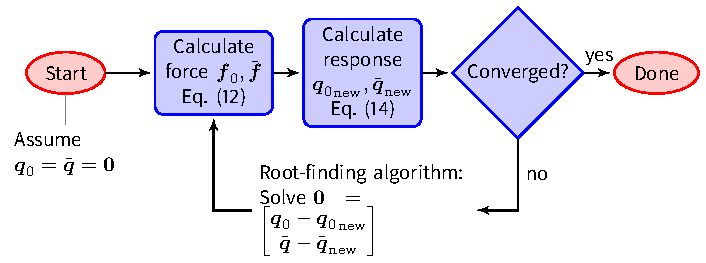
\includegraphics{tikz/solution}

  \noindent where the iteration is controlled by a numerical multi-dimensional
  root-finding algorithm. In the first case, finding the structural response,
  there is little difficulty in finding the solution since the structural
  response is linear, but in the later cases and in general an iterative
  numerical solution is needed. The `hybr' method implemented in SciPy
  \citep{SciPy} was used.

\subsection{Non-linear reference results}
\label{sec:appendix-method-nonlinear}

The non-linear reference results were found from numerical simulation of a Blade
Element Momentum (BEM) aerodynamic model combined with a flexible multi-body
dynamics code described and validated in \citet{lupton_frequencydomain_2015}.

Simulations were run for the conditions listed in Table~\ref{tab:test-grid} for
the minimum of \SI{60}{\second} or \num{5}~cycles, leading to the following
parameters:

{ \centering
  \begin{tabular}{lll}
    $\SI{0.03}{\radian\per\second}$ &
    $t_{\mathup{max}} = \SI{1987}{\second}$ &
    $\Delta t = \SI{1}{\second}$ \\
  %
    $\SI{0.10}{\radian\per\second}$ &
    $t_{\mathup{max}} = \SI{628}{\second}$ &
    $\Delta t = \SI{1}{\second}$ \\
  %
    $\SI{0.32}{\radian\per\second}$ &
    $t_{\mathup{max}} = \SI{199}{\second}$ &
    $\Delta t = \SI{0.1}{\second}$ \\
  %
    $\SI{1.00}{\radian\per\second}$ &
    $t_{\mathup{max}} = \SI{63}{\second}$ &
    $\Delta t = \SI{0.1}{\second}$ \\
  %
    $\SI{3.16}{\radian\per\second}$ &
    $t_{\mathup{max}} = \SI{60}{\second}$ &
    $\Delta t = \SI{0.01}{\second}$ \\
  \end{tabular} \par
}
The first parts of the simulations are discarded, removing initial
transients, and only the final cycle is used. 

\section{Additional aerodynamic force results}
\label{sec:appendix-aero-force}

\begin{figure}
  \centering
  \hspace*{-1.5cm}\includegraphics{figures/linearisation_sine_examples}
  \caption{Example linearisation results for rotor loads and blade tip
    in-plane (IP) and out-of-plane (OOP) deflections, plotted over one
    cycle of harmonic wind speed input
    ($8\pm5$~\si{\metre\per\second}). The columns correspond to wind
    speed variations of different frequencies.}
\label{fig:hlin-example-sinusoids}
\end{figure}

\begin{table}
  \centering
  \caption{Error of linearisations, as shown in
    Figures~\protect\ref{fig:hlin-errors-rms-1}--\protect\ref{fig:hlin-errors-rms-2}. The
    maximum error for various amplitudes of wind speed variation $A$ is shown.}
  \label{tab:hlin-errors-peak}
  \begin{tabular}{lrrrr}
    \toprule
     & Out-of-plane & In-plane & Rotor & Rotor \\
     & defl. & defl. & thrust & torque \\
    \midrule
    \multicolumn{4}{l}{Mean wind speed \SI{8}{\metre\per\second}} \\[1em]
    \multicolumn{4}{l}{Harmonic:} \\
    $A<$ \SI{ 1 }{\metre\per\second}& \SI{ 0.5 }{\%}& \SI{ 2.0 }{\%}& \SI{ 0.5 }{\%}& \SI{ 2.2 }{\%}\\
    $A<$ \SI{ 2 }{\metre\per\second}& \SI{ 1.0 }{\%}& \SI{ 2.1 }{\%}& \SI{ 1.0 }{\%}& \SI{ 2.6
 }{\%}\\
    $A<$ \SI{ 3 }{\metre\per\second}& \SI{ 1.1 }{\%}& \SI{ 2.1 }{\%}& \SI{ 1.5 }{\%}& \SI{ 3.0 }{\%}\\
    $A<$ \SI{ 4 }{\metre\per\second}& \SI{ 1.6 }{\%}& \SI{ 2.1 }{\%}& \SI{ 3.5 }{\%}& \SI{ 4.8 }{\%}\\
    $A<$ \SI{ 5 }{\metre\per\second}& \SI{ 2.8 }{\%}& \SI{ 2.6 }{\%}&
                                                                        \SI{ 5.7 }{\%}& \SI{ 8.4 }{\%}\\
    \multicolumn{4}{l}{Tangent:} \\
    $A<$ \SI{ 1 }{\metre\per\second}& \SI{ 1.6 }{\%}& \SI{ 2.3 }{\%}& \SI{ 1.4 }{\%}& \SI{ 2.1 }{\%}\\
    $A<$ \SI{ 2 }{\metre\per\second}& \SI{ 4.8 }{\%}& \SI{ 3.0 }{\%}& \SI{ 4.5 }{\%}& \SI{ 5.2 }{\%}\\
    $A<$ \SI{ 3 }{\metre\per\second}& \SI{ 7.4 }{\%}& \SI{ 5.7 }{\%}& \SI{ 8.0 }{\%}& \SI{ 10.1 }{\%}\\
    $A<$ \SI{ 4 }{\metre\per\second}& \SI{ 10.1 }{\%}& \SI{ 9.7 }{\%}& \SI{ 14.4 }{\%}& \SI{ 19.3 }{\%}\\
    $A<$ \SI{ 5 }{\metre\per\second}& \SI{ 14.5 }{\%}& \SI{ 16.7 }{\%}& \SI{ 24.1 }{\%}& \SI{ 34.1 }{\%}\\[1em]

    \midrule
    \multicolumn{4}{l}{Mean wind speed \SI{16}{\metre\per\second}} \\[1em]
    \multicolumn{4}{l}{Harmonic:} \\
$A<$ \SI{ 1 }{\metre\per\second}& \SI{ 0.5 }{\%}& \SI{ 3.4 }{\%}& \SI{ 0.5 }{\%}& \SI{ 2.6 }{\%}\\
$A<$ \SI{ 2 }{\metre\per\second}& \SI{ 0.5 }{\%}& \SI{ 3.4 }{\%}& \SI{ 0.5 }{\%}& \SI{ 2.7 }{\%}\\
$A<$ \SI{ 3 }{\metre\per\second}& \SI{ 0.7 }{\%}& \SI{ 3.4 }{\%}& \SI{ 0.6 }{\%}& \SI{ 2.8 }{\%}\\
$A<$ \SI{ 4 }{\metre\per\second}& \SI{ 0.7 }{\%}& \SI{ 3.4 }{\%}& \SI{ 0.7 }{\%}& \SI{ 3.0 }{\%}\\
$A<$ \SI{ 5 }{\metre\per\second}& \SI{ 0.7 }{\%}& \SI{ 3.4 }{\%}& \SI{ 0.8 }{\%}& \SI{ 3.3 }{\%}\\[1em]

    \multicolumn{4}{l}{Tangent:} \\
    $A<$ \SI{ 1 }{\metre\per\second}& \SI{ 0.5 }{\%}& \SI{ 3.4 }{\%}& \SI{ 0.5 }{\%}& \SI{ 2.5 }{\%}\\
    $A<$ \SI{ 2 }{\metre\per\second}& \SI{ 0.5 }{\%}& \SI{ 3.4 }{\%}& \SI{ 0.9 }{\%}& \SI{ 2.5 }{\%}\\
    $A<$ \SI{ 3 }{\metre\per\second}& \SI{ 1.3 }{\%}& \SI{ 3.6 }{\%}& \SI{ 1.4 }{\%}& \SI{ 2.5 }{\%}\\
    $A<$ \SI{ 4 }{\metre\per\second}& \SI{ 1.3 }{\%}& \SI{ 3.6 }{\%}& \SI{ 2.5 }{\%}& \SI{ 3.9 }{\%}\\
    $A<$ \SI{ 5 }{\metre\per\second}& \SI{ 1.3 }{\%}& \SI{ 3.6 }{\%}& \SI{ 3.5 }{\%}& \SI{ 6.0 }{\%}\\

    \bottomrule
  \end{tabular}
\end{table}

Figure~\ref{fig:hlin-example-sinusoids} shows a different view of the results in
Figure~\ref{fig:hlin-example-loops} by plotting against time.
Table~\ref{tab:hlin-errors-peak} gives numeric data shown in
Figures~\ref{fig:hlin-errors-rms-1}--\ref{fig:hlin-errors-rms-2}.

% \begin{figure}
%   \centering
%   \includegraphics[width=\linewidth]{tmp_figures/hlin_error_peak.png}
%   \caption{Peak-peak error between linearised and nonlinear results,
%     normalised by nonlinear result standard deviation.}
% \label{fig:hlin-errors-peak}
% \end{figure}

% \begin{figure}
%   \centering
%   \includegraphics[width=\linewidth]{tmp_figures/hlin_error_rms_tangent_rel_harmonic.png}
%   \includegraphics[width=\linewidth]{tmp_figures/hlin_error_peak_tangent_rel_harmonic.png}
%   \caption{Factor of improvement of harmonic linearisation relative to
%     tangent linearisation, measured by Equation~\eqref{eq:150}.}
% \label{fig:hlin-errors-rms-rel}
% \end{figure}

\section{Additional control linearisation results}
\label{sec:appendix-control-results}

\begin{figure}
  \centering
  \hspace*{-1cm}\includegraphics{figures/control_linearisation_examples_lowfreq}
  \caption{Comparison of linearised and non-linear results for harmonic
    wind speed input varying at \SI{0.10}{\radian\per\second}. Dotted
    lines show mean values. It was not possible to find a solution
    with a mean wind speed of \SI{10}{\metre\per\second}; see text for
    discussion.}
\label{fig:control-lin-lowfreq}
\end{figure}

\begin{figure}
  \centering
  \hspace*{-1cm}\includegraphics{figures/control_linearisation_examples_highfreq}
  \caption{Comparison of linearised and non-linear results for harmonic
    wind speed input varying at \SI{1.00}{\radian\per\second}. Dotted
    lines show mean values.}
\label{fig:control-lin-highfreq}
\end{figure}

Figures~\ref{fig:control-lin-lowfreq}--\ref{fig:control-lin-highfreq} show
similar results to those shown in Figure~\ref{fig:control-lin-midfreq}, for a
lower and a higher frequency respectively.

\end{document}

%%% Local Variables: 
%%% mode: latex
%%% TeX-engine: luatex
%%% TeX-master: t
%%% End: 
